\documentclass[pdftex,12pt,a4paper]{article}
\usepackage[pdftex]{graphicx}
\usepackage{xcolor}
\usepackage{marginnote}
\usepackage{enumitem}
\usepackage[bottom=1.5cm, outer=5cm, inner=2cm, heightrounded,
marginparwidth=4cm, marginparsep=0.5cm]{geometry}

\begin{document}
    % Custom title page
    \begin{titlepage}
        \begin{center}
            
\includegraphics[width=5cm]{figures/kulogo}\\[1cm]
            {\Large \bfseries
                Spring 2014\\
                Computer Networks\\
                CMPE323\\[1cm]
            }
            {\large \bfseries
                \noindent Laboratory Experiment No. 8: Introduction to NAPT\\[1cm]
            }
        \end{center}

        \noindent \textbf{Aims and Objectives:}
            \begin{itemize}[leftmargin=4cm]
                \item Introducing Network Address and Port Translation (NAPT).
            \end{itemize}
            \vspace{0.5cm}

        \noindent \textbf{Materials Required:}
            \begin{itemize}[leftmargin=4cm]
                \item IP routers,
                \item PCs with Ethernet adapters,
                \item and straight-through/crossover/rollover cables.
            \end{itemize}
            \vspace{0.5cm}

        \noindent \textbf{Change Log:}
            \begin{itemize}[leftmargin=4cm]
                \item 15-4-2014: original document -- mkhonji.
                \item 23-4-2014: added PC3, changed lab no. from 7 to 8 -- mkhonji.
            \end{itemize}
    \end{titlepage}
    \newpage

    % Lab script content
    \section{Introduction}
        IPv4 addresses are 32 bit numbers which gives us $2^{32}$ unique
        addresses (some of which are not usable for Internet communication as
        they are reserved for other purposes).

        Although the $2^{32}$ addresses might seem to be large at first, the
        amount of  growth that the Internet has experienced demands even a
        larger address space. This became apparent in the 1980s when the fears
        from depleted IPv4 address surfaced.

        In order to handle the shortage in the IPv4 address space, a number of
        solutions were proposed at the same time, such as:
        \begin{itemize}
            \item Larger IP address space (e.g. IPv6).
            \item Classless Inter-Domain Routing instead of classfull routing.
            \item Network Address Translation (NAT).
        \end{itemize}

        It is highly likely that if you used the Internet, you have already
        used Network Address and Port Translation (NAPT), which is the most
        wide-spread NAT type.

        There are other types of NAT, such as: static NAT, dynamic NAT, source NAT,
        destination NAT, \ldots. However, in this lab, we will only focus on the most
        common NAT type which is NAPT.

        \textbf{Note:} it is important to note that although the original
        motives for NAT were to postpone the depletion of IPv4 addresses,
        NAT is used for many other scenarios as well, such as solving some IP
        address conflict scenarios and IPv4 to IPv6 migration.

        \subsection{NAPT}
            In order to save public IP addresses, two perquisites are needed:
            \begin{itemize}
                \item Private IP addresses.
                \item , and a NAPT-ready device (often integrated in routers).
            \end{itemize}

            \subsubsection{Private IPv4 addresses}
                RFC1918 defines the following ranges (or blocks) of private IP
                addresses:
                \begin{itemize}
                    \item 10.0.0.0 -- 10.255.255.255 (named as the 24-bit private
                        address block, historically known as the class A private IP
                        address block).
                    \item 172.16.0.0 -- 172.31.255.255 (named as the 20-bit private
                        address block, historically known as the class B private IP
                        address block)
                    \item 192.168.0.0 -- 192.168.255.255 (named as the 16-bit
                        private address block, historically known as the class C
                        address block).
                \end{itemize}

                The interesting property of private IP addresses is that they
                are not used in the Internet but rather reserved for local
                networks only.

                This way, different local networks can re-use the same IP
                address blocks as long as they are not inter-connected
                directly without address translation.

                For example, if 100 computers in company $X$ and 100 other
                computers in company $Y$ demand access to the Internet,
                they can all use the same address block (e.g. 24-bit block) and
                till being able to access the Internet via NAPT (as covered in
                the next section). This way, we can greatly save IPv4
                addresses.

            \subsubsection{NAPT-ready devices}
                This subsection will explain how a NAPT device can allow many
                computers with private IP addresses access the Internet using
                only a single public IP address.

                As depicted in Figure \ref{fig:intro}, a number of computers in
                a private network (one that uses the 10.0.0.0/8 24-bit block) require
                access to the Internet via some Internet  Service Provider
                (ISP).
                

                \begin{figure}[tbh]
                    \centering
                    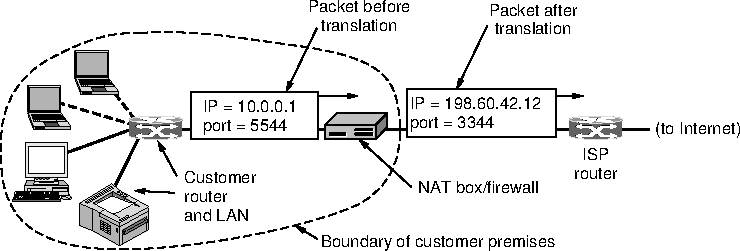
\includegraphics[width=0.9\textwidth]{figures/intro}
                    \caption{A Network Address and Port Translation (NAPT)
                        scenario --- Source: Computer Networks 5$^{th}$ Edition, 2010, by
                        Andrew S. Tanenbaum and David J. Wetherall, page 453.}
                    \label{fig:intro}
                \end{figure}

                In order to perform NAPT, the following steps are performed:
                \begin{enumerate}
                    \item A computer with the IP 10.0.0.1 in the private
                        network 10.0.0.0/8 sends a packet to
                        some resource in the Internet (e.g. TCP request to port
                        80 on 173.194.39.39 which is a Google web server).
                        Therefore, the source IP address is 10.0.0.1, the source TCP
                        port is some dynamically chosen number by the
                        computer's TCP implementation (we will assume the
                        source port is 50,000), the destination IP
                        address is 173.194.39.39 (the IP of some Google web
                        server), and the destination port number is 80 (often
                        used for HTTP web servers).
                    \item Some Internet Service Provider (ISP) has assigned a
                        single public IP address to the local network, and this
                        IP address is 198.60.42.12.
                    \item As the computer is not connected to any network that
                        has the IP address 173.194.39.39, it will forward the
                        packet to its default gateway (the local router).
                    \item Before the packet is forwarded to the ISP router (to
                        deliver the packet to its destination), NAPT
                        translation occurs as follows:
                        \begin{enumerate}
                            \item The packet is modified such that its source IP address 10.0.0.1 is changed to
                                198.60.42.12.
                            \item An entry is added to the \emph{NAT
                                translation table} of the NAPT device
                                which maps the source IP address 10.0.0.1 and
                                the source TCP port 50,000 to the public IP
                                address 198.60.42.12 with the same source TCP
                                port 50,000. \textbf{Note:} if the combination
                                198.60.42.12:50000 exists in the table, the
                                port is translated to some other port number
                                such as 50,001. The goal is ensuring that
                                different connections have unique
                                \texttt{publicIP:port} mappings.
                        \end{enumerate}
                    \item The modified packet is sent to the ISP which in turn
                        forwards it to other routers that will ultimately reach
                        the target destination 173.194.39.39 on the TCP 80. The
                        receiver of this packet will notice that the source IP
                        address is 198.60.42.12 (instead of 10.0.0.1). In other
                        words, we can think of the NAPT translation entry as
                        \texttt{TCP: 10.0.0.1:50000 --> 198.60.42.12:50000}.
                    \item If the Google web server 198.60.42.12 responded back
                        (which most likely it will given how HTTP works), it
                        will send a packet with a destination IPv4 address of
                        198.60.42.12 and a destination port number of 50,000.
                    \item When the NAPT device gets the response from the
                        Google web server, the NAPT device will lookup its NAT
                        translation table for a match for
                        \texttt{198.60.42.12:5000}.
                    \item The NAT table lookup will succeed and will identify
                        that the combination \texttt{198.60.42.12:50000} was
                        originally \texttt{10.0.0.1:5000}.
                    \item the NAPT device will reverse the translation back by
                        modifying the destination IP address 198.60.42.12 and
                        port 50,000 back to the original one which are the IP
                        0.0.0.1 and the port 50,000.
                \end{enumerate}

                This way, theoretically, each public IP address can be used by
                $2^{16}$ TCP or UDP connections. The number $2^{16}$ is due to
                the fact that TCP and UDP port numbers are 16 bit numbers.


    \section{Lab Preparation}
        \begin{enumerate}
            \item Erase the configuration of
                \texttt{R1}\footnote{\texttt{enable}, \texttt{erase
                startup-config}, \texttt{reload}, and make sure to answer
                \texttt{no} to all yes/no questions while hitting \emph{enter} for
                all \texttt{confirm} prompts.} and reboot \texttt{PC1},
                \texttt{PC2} and \texttt{PC3}.
            \item Physically connect and configure IP addresses of the
                router\footnote{\texttt{enable}, \texttt{configure terminal},
                \texttt{interface Gi0/0}, \texttt{ip address <ip\_address>
                <subnet\_mask>}, \texttt{no shutdown}.} and the
                PCs\footnote{\texttt{ifconfig eth0
                <ip\_address>/<netmask\_bits>}} as depicted in Figure
                \ref{fig:labtop}.

                \begin{figure}[tbh]
                    \centering
                    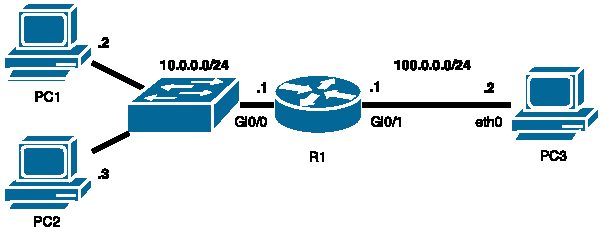
\includegraphics[width=0.9\textwidth]{figures/npat}
                    \caption{Lab topology.}
                    \label{fig:labtop}
                \end{figure}

           \item Add default routes\footnote{\texttt{route add -net
               0.0.0.0/0 gw <nexthop\_ip>}} to \texttt{PC1}, \texttt{PC2} and \texttt{PC3}.

           \item Run Wireshark on all the PCs.

           \item Using the \texttt{nc}\footnote{\texttt{nc -l -p <port> -s
               <ip\_address>}} command run three applications on \texttt{PC3} that
               listen on TCP ports as follows:
                \begin{itemize}
                    \item Application 1: listen on IP 100.0.0.2 and TCP port 100.
                \end{itemize}

           \item Using the \texttt{nc}\footnote{\texttt{nc -l -u -p <port> -s
               <ip\_address>}} command run three applications on \texttt{PC3} that
               listen on UDP ports as follows:
                \begin{itemize}
                    \item Application 2: listen on IP 100.0.0.2 and UDP port 100.
                \end{itemize}
        \end{enumerate}

    \section{Lab experiments}
        \subsection{Configuring NAPT on \texttt{R1}}
            Connect to \texttt{R1} using the console port and perform the
            following configurations:
            \begin{itemize}
                \item Configure an Access-Control List (ACL) that specifies
                    which IP addresses to be matched. Note that
                    \texttt{0.0.0.255} is called a \emph{wild-card mask} which
                    is semantically the same as the subnet mask
                    \texttt{255.0.0.0}. Note that a wild-card mask is the
                    opposite of a subnet mask. The reason for such difference
                    in the Cisco IOS is historical and beyond the lab's scope.
                    \begin{enumerate}
                        \item \texttt{enable}.
                        \item \texttt{config terminal}.
                        \item \texttt{ip access-list standard <list\_name>}.
                        \item \texttt{permit 10.0.0.0 0.0.0.255}.
                        \item \texttt{end}.
                    \end{enumerate}
                \item Configure \texttt{R1} so that it knows which interface
                    faces the inside (possibly private) network and which
                    interface faces the outside (possibly public) network.
                    \begin{enumerate}
                        \item \texttt{enable}.
                        \item \texttt{config terminal}.
                        \item \texttt{int gi0/0}.
                        \item \texttt{ip nat inside}.
                        \item \texttt{exit}.
                        \item \texttt{int gi0/1}.
                        \item \texttt{ip nat outside}.
                        \item \texttt{ip nat inside}.
                        \item \texttt{end}.
                    \end{enumerate}
                \item Enable NAPT such that, for any IP packet that enters an
                    inside interface that is also going to be routed to the
                    outside interface, will have the NAPT translation applied
                    against (as described earlier).
                    \begin{enumerate}
                        \item \texttt{enable}.
                        \item \texttt{config terminal}.
                        \item \texttt{ip nat inside source list <list\_name> interface
                            fa0/1 overload}.
                        \item \texttt{end}.
                    \end{enumerate}
            \end{itemize}

            \subsection{Analysing packets}
                \begin{flushright}
                    \textbf{[100 points]}\marginnote{\small \textbf{Note:} when done, show your
                    work to the lab engineer for grading purposes.}
                \end{flushright}

                While monitoring Wireshark instances on relevant PCs, use
                \texttt{PC1} to perform the following tasks:
                \begin{enumerate}
                    \item View the \emph{NAT translation table} of \texttt{R1}
                        by \texttt{show ip nat translations}. It should be
                        empty.

                    \item Using PC1, connect to \texttt{PC3}'s \texttt{nc} server that is
                        listening on the TCP port 100 such that the source port is
                        \texttt{50000}. Use the command \texttt{nc -p 5000
                        100.0.0.2 100}. By observing Wireshark, note down the following
                        information:
                        \begin{itemize}
                            \item Source IP, layer 4 protocol, source port, destination IP and
                                destination port numbers as it appears on
                                \texttt{PC1}'s Wireshark instance.
                            \item Source IP, layer 4 protocol, source port, destination IP and
                                destination port numbers as it appears on
                                \texttt{PC3}'s Wireshark instance.
                        \end{itemize}

                    \item View the \emph{NAT translation table} of \texttt{R1}
                        by \texttt{show ip nat translations} and compare its
                        content against the information that you have gathered
                        above. You should see new entries. How do the entries
                        relate to the data that you have observed in the
                        previous point?

                    \item Using PC1, connect to \texttt{PC3}'s \texttt{nc} server that is
                        listening on the UDP port 100 such that the source port is
                        \texttt{50000}. Use the command \texttt{nc -u -p 5000
                        100.0.0.2 100}. By observing Wireshark, note down the following
                        information:
                        \begin{itemize}
                            \item Source IP, layer 4 protocol, source port, destination IP and
                                destination port numbers as it appears on
                                \texttt{PC1}'s Wireshark instance.
                            \item Source IP, layer 4 protocol, source port, destination IP and
                                destination port numbers as it appears on
                                \texttt{PC3}'s Wireshark instance.
                        \end{itemize}

                    \item View the \emph{NAT translation table} of \texttt{R1}
                        by \texttt{show ip nat translations} and compare its
                        content against the information that you have gathered
                        above. You should see new entries. How do the entries
                        relate to the data that you have observed in the
                        previous point?

                    \item Using PC2, connect to \texttt{PC3}'s \texttt{nc} server that is
                        listening on the TCP port 100 such that the source port is
                        \texttt{50000}. Use the command \texttt{nc -p 5000
                        100.0.0.2 100}. By observing Wireshark, note down the following
                        information:
                        \begin{itemize}
                            \item Source IP, layer 4 protocol, source port, destination IP and
                                destination port numbers as it appears on
                                \texttt{PC2}'s Wireshark instance.
                            \item Source IP, layer 4 protocol, source port, destination IP and
                                destination port numbers as it appears on
                                \texttt{PC3}'s Wireshark instance.
                        \end{itemize}

                    \item View the \emph{NAT translation table} of \texttt{R1}
                        by \texttt{show ip nat translations} and compare its
                        content against the information that you have gathered
                        above. You should see new entries. How do the entries
                        relate to the data that you have observed in the
                        previous point?

                    \item Using PC2, connect to \texttt{PC3}'s \texttt{nc} server that is
                        listening on the UDP port 100 such that the source port is
                        \texttt{50000}. Use the command \texttt{nc -u -p 5000
                        100.0.0.2 100}. By observing Wireshark, note down the following
                        information:
                        \begin{itemize}
                            \item Source IP, layer 4 protocol, source port, destination IP and
                                destination port numbers as it appears on
                                \texttt{PC2}'s Wireshark instance.
                            \item Source IP, layer 4 protocol, source port, destination IP and
                                destination port numbers as it appears on
                                \texttt{PC3}'s Wireshark instance.
                        \end{itemize}

                    \item View the \emph{NAT translation table} of \texttt{R1}
                        by \texttt{show ip nat translations} and compare its
                        content against the information that you have gathered
                        above. You should see new entries. How do the entries
                        relate to the data that you have observed in the
                        previous point?

                \item Then answer the following questions:
                    \begin{itemize}
                        \item Which IP addresses are being translated (source
                            or destination)?
                        \item Which port numbers are being translated (source
                            or destination)?
                        \item What are the cases when the translated port
                            numbers are identical to the pre-translation port
                            numbers?
                        \item What are the cases when the translated port
                            numbers are different to the pre-translation port
                            numbers?
                        \item How can NAPT save IPv4 addresses?
                    \end{itemize}
                \end{enumerate}

        \subsection{Extra questions (not graded)}
            \begin{itemize}
                \item For protocols that do not use TCP or UDP port numbers,
                    how can NAPT function? For example, ICMP does not rely on
                    TCP nor UDP yet it functions correctly. In other words, how
                    can the NAPT device identify which ICMP Echo-Reply is for
                    which ICMP Echo (request) from which PC or process?
                \item What is the behaviour of a Cisco router if its NAT
                    translation table is full?
            \end{itemize}

\end{document}
